%%%%%%%%%%%%%%%%%%%%%%%%%%%%%%%%%%%%%%%%%%%%%%%%%%%%%%%%%%%%%%%%%%%%%%%%%%%%%%%
\subsection{Characteristics of Individual Bees}
%%%%%%%%%%%%%%%%%%%%%%%%%%%%%%%%%%%%%%%%%%%%%%%%%%%%%%%%%%%%%%%%%%%%%%%%%%%%%%%
What is the distribution of values within the colony.
Are all bees the same or is there a big difference, maybe indicating two groups to functional groups or different behaviour
Question: With how many other bees does a bee interact? Is this the same for all bees, what is the distribution?\\



The degree of a bee represents the number of other bees this individual interacts with.
Figure~\ref{fig:n3-degree} indicates a bimodal degree distribution, with a borderline at about $0.4$. This indicates the presence of two groups of bees, one group interacts with less than 40\% of the population, and the second group with at least 40\% (local peak at 80\%).
The degree distribution does not follow a power law, but rather a normal distribution. Therefore most bees have the same number of links. This indicates the absence of hubs\footnote{Hubs are highly connected nodes having a large number of links.}, meaning a few bees beeing highly connected. 

Degree and detection frequency are positively correlated, the higher the degree the higher is the detection frequency.

The higher the degree the higher the detection frequency. Bees staying in the hive, are detected more often then for example foragers. Those bees have of course more time to gather links to other bees.

Strength


Degree, Strength and Local Clustering Coefficient and \\
Betweenness and Closeness Centrality\\
\\
bimodal degree distribution\\
type of network: no scale free\\
todo plot in relation to age of bees\\
todo plot in relation to detection frequency\\

\begin{figure}[!htb]
	\centering
	\begin{subfigure}[b]{1.0\textwidth}
	\centering
	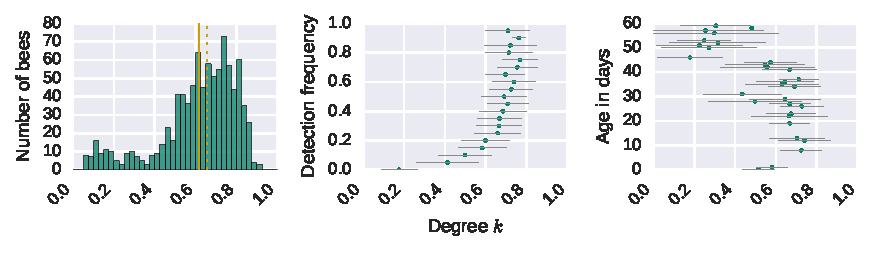
\includegraphics[width=1.0\textwidth]{Figures/n3-stat-degreeAgeDetF.pdf}
	\caption[Degree]{\textbf{Degree}}
	\label{fig:n3-degree}
	\end{subfigure}
	\begin{subfigure}[b]{1.0\textwidth}
	\centering
	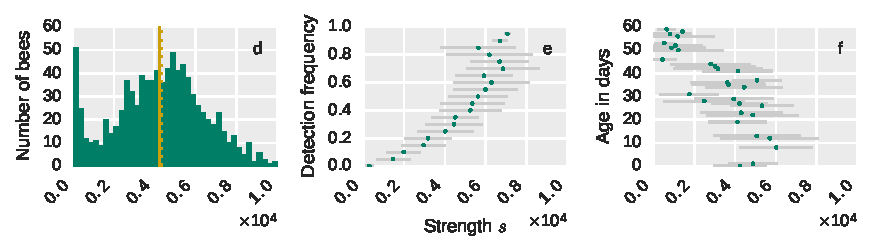
\includegraphics[width=1.0\textwidth]{Figures/n3-stat-strengthAgeDetF.pdf}
	\caption[Strength]{\textbf{Strength}}
	\label{fig:n3-strength}
	\end{subfigure}
	\begin{subfigure}[b]{1.0\textwidth}
	\centering
	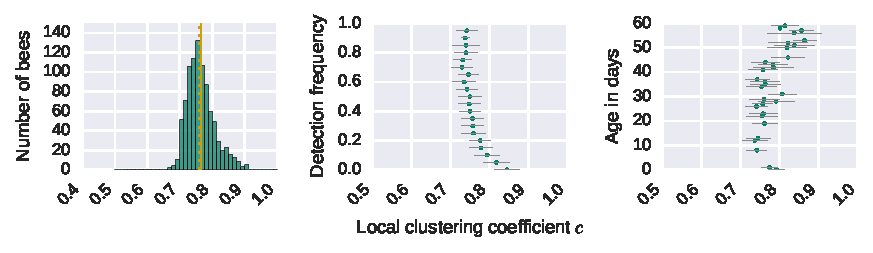
\includegraphics[width=1.0\textwidth]{Figures/n3-stat-lccAgeDetF.pdf}
	\caption[Local clustering coefficient]{\textbf{Local clustering coefficient}}
	\label{fig:n3-lcc}
	\end{subfigure}
	\caption[Degree, strength and local clustering coefficient (LCC)]{\textbf{Degree, strength and local clustering coefficient (LCC) in relation to age and detection frequency} xxx}
	\label{fig:n3-degreeStrLCC}
\end{figure}


[TODO]\\
in relation to age and detection frequency\\
closeness\\
betweenness\\

\begin{figure}[!htb]
	\centering
	\begin{subfigure}[b]{1.0\textwidth}
	\centering
	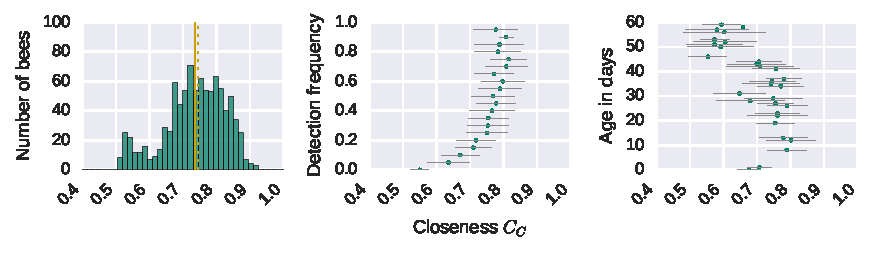
\includegraphics[width=1.0\textwidth]{Figures/n3-stat-closenessAgeDetF.pdf}
	\caption[Closeness Centrality]{\textbf{Closeness Centrality}}
	\label{fig:n3-closeness}
	\end{subfigure}
	\begin{subfigure}[b]{1.0\textwidth}
	\centering
	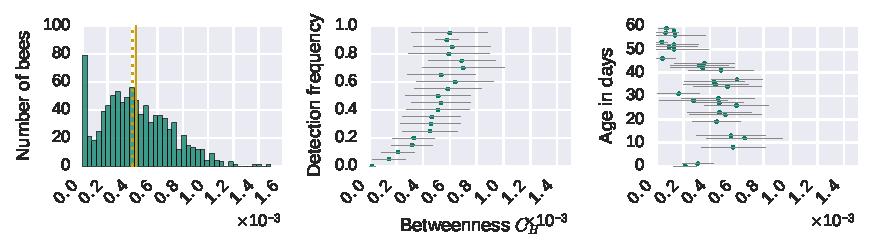
\includegraphics[width=1.0\textwidth]{Figures/n3-stat-betweenAgeDetF.pdf}
	\caption[Betweeness Centrality]{\textbf{Betweeness Centrality}}
	\label{fig:n3-between}
	\end{subfigure}
	\caption[Centrality]{\textbf{Centrality in relation to age and detection frequency} xxx}
	\label{fig:n3-centrality}
\end{figure}
